\chapter{General framework} \label{s:fra}

\minitoc

\section{Introduction}

This chapter presents succinctly the spacetime framework used in these lectures
(Sec.~\ref{s:fra:spacetime})
and recalls useful basic concepts, such as worldlines of particles and observers
(Sec.~\ref{s:fra:worldlines} and \ref{s:fra:measure}).
In a great part of these lectures, we shall assume that the theory of gravitation is general
relativity; this means that the spacetime metric obeys the Einstein equation,
which is recalled in Sec.~\ref{s:fra:Einstein_eq}.

This chapter is by no means an introduction to general relativity. We
recommend the textbooks \cite{Carro04,Choqu15,DerueU18,Hartl03,MisneTW73,Strau13,Wald84} in this
respect, as well as \cite{DerueU14,Gourg14,Langl13} for the French-speaking reader.
The reader might also find useful to start the reading by Appendix~\ref{s:bas}, which
recaps the concepts from differential geometry employed in the main text.

\section{Spacetime} \label{s:fra:spacetime}

\subsection{General settings}

In these lectures we consider a $n$-dimensional \defin{spacetime}\index{spacetime},
i.e. a pair $(\M, \w{g})$, where $\M$ is a $n$-dimensional smooth manifold, with $n\geq 2$, and $\w{g}$ is a Lorentzian metric on $\M$. In many parts, $n$ will be set to 4
--- the standard spacetime dimension --- but we shall also consider spacetimes with
$n\neq 4$.

The precise definition and basic properties of a \emph{smooth manifold} are recalled
in Appendix~\ref{s:bas}. Here let us simply say that, in loose terms,
a \defin{manifold}\index{manifold} $\M$ of dimension $n$ is a ``space'' that \emph{locally} resembles $\R^n$,
i.e. can be described by a $n$-tuple of coordinates $(x^1,\ldots,x^n)$. However, globally,
$\M$ can be very different from $\R^n$, in particular regarding its topology. It could also happen
that many coordinate systems are required to cover $\M$, while a single one is obviously
sufficient for $\R^n$.

\begin{figure}
\centerline{\includegraphics[width=0.6\textwidth]{fra_manifold.pdf}}
\caption[]{\label{f:fra:manifold} \footnotesize
A smooth manifold $\M$: the infinitesimal vector $\D\w{x}$ connects the nearby points $p$ and $q$ and thus
can thought as a displacement within the manifold, while the finite vector $\w{v}$ does not correspond to
any displacement in the manifold and ``lives'' in the tangent space $T_p\M$.}
\end{figure}


The smooth structure endows the manifold
with the concept of \defin{infinitesimal displacement vectors}\index{infinitesimal! displacement vector}\index{vector!infinitesimal --} $\D\w{x}$, which connect infinitely
close points of $\M$ (cf. Fig.~\ref{f:fra:manifold} and Sec.~\ref{s:bas:vectors} of Appendix~\ref{s:bas}). However, for finitely separated points, there is no
longer the concept of connecting vector (contrary for instance to points in $\R^n$).
In other words, vectors on $\M$ do not live in the manifold but in the
\defin{tangent spaces}\index{tangent!space} $T_p\M$, which are defined at each point $p\in\M$. Each  $T_p\M$
is a $n$-dimensional vector space, which is generated for instance by the infinitesimal displacement
vectors along the $n$ coordinate lines of some coordinate system.
Unless explicitly specified, we assume that $\M$ is an orientable manifold (cf. Sec.~\ref{s:bas:Levi-Civita_tensor}).

The full definition of the \defin{metric tensor} $\w{g}$ is given in Sec.~\ref{s:bas:pRiemManif} of
Appendix~\ref{s:bas}. At each point $p\in\M$, $\w{g}$ induces a (non positive definite)
scalar product on $T_p\M$, which we shall denote by a dot:
\be
    \forall (\w{u},\w{v})\in T_p\M\times T_p\M, \quad
        \w{u}\cdot\w{v} := \w{g}(\w{u}, \w{v}) .
\ee
Given a coordinate system $(x^\alpha)$, the components of $\w{g}$ with respect
to it are the $n^2$ scalar fields $(g_{\alpha\beta})$ such that [cf. Eq.~(\ref{e:bas:g_components_dx})]
\be \label{e:fra:g_components_dx}
    \encadre{ \w{g} = g_{\alpha\beta} \, \dd x^\alpha \dd x^\beta },
\ee
where $\dd x^\alpha$ is the differential 1-form of $x^\alpha$ (cf. Sec.~\ref{s:bas:linear_form})
and the notation $\dd x^\alpha \dd x^\beta$ stands for the symmetric tensor product
defined by Eq.~(\ref{e:bas:sym_tensor_prod}).
The scalar square $\D s^2$ of an infinitesimal
displacement vector $\D\w{x} = \D x^\alpha \wpar_\alpha$ is expressed in
terms of the components $(g_{\alpha\beta})$ by the line element\index{line!element}
formula
\be \label{e:fra:line_element}
    \D s^2 := \w{g}(\D\w{x},\D\w{x}) = g_{\alpha\beta} \, \D x^\alpha \, \D x^\beta .
\ee
This formula follows from Eq.~(\ref{e:fra:g_components_dx}) via the identity
$\langle\dd x^\alpha,\D\w{x} \rangle =  \D x^\alpha$ [Eq.~(\ref{e:bas:dxa_dxa})].

\begin{remark}
In this book, we shall use the bilinear form identity (\ref{e:fra:g_components_dx}) rather than
the line element (\ref{e:fra:line_element}) to present a metric (cf. Box.~3.2 of MTW \cite{MisneTW73}
for a discussion). It turns out to be more convenient when various metric tensors are
involved, the notation $\D s^2$ being then ambiguous.
\end{remark}

The fact that the signature of $\w{g}$ is Lorentzian, i.e.
\be
\mathrm{sign}\; \w{g} = (-,\underbrace{+,\ldots,+}_{\mbox{\small $n-1$ times}}),
\ee
implies that at each point $p\in\M$, there are privileged directions,
along which the line element (\ref{e:fra:line_element}) vanishes; they
form the so-called \defin{null cones}\index{null!cone}
or \defin{light cones}\index{light!cone} (cf. Fig.~\ref{f:fra:lorentz_manifold}).
The null cones constitute an absolute structure of spacetime, independent from any observer.
A vector at a point $p\in\M$ that is either timelike or null
(cf. Sec.~\ref{s:bas:signature})
is said to be \defin{causal}\index{causal!vector}.
It lies necessarily inside the null cone at $p$ (timelike vector) or along it (null vector).

\begin{figure}
\centerline{\includegraphics[width=0.6\textwidth]{fra_lorentz_manifold.pdf}}
\caption[]{\label{f:fra:lorentz_manifold} \footnotesize
A Lorentzian manifold $(\M,\w{g})$: at each point, the metric tensor $\w{g}$
defines privileged directions: those lying in the null cone at $p$.}
\end{figure}

\subsection{Time orientation} \label{s:fra:time_orientation}

When dealing with black hole spacetimes, it is very important to have clear
concepts of ``past'' and ``future''. Therefore, we assume
that the spacetime $(\M, \w{g})$ is \emph{time-orientable}, i.e. that it is possible to divide \emph{continuously} all causal (i.e. timelike or null) vectors into
two classes, the \emph{future-directed} ones and the \emph{past-directed} ones.
More precisely, at each tangent space $T_p\M$, we may split the causal
vectors in two classes by declaring that two causal
vectors belong to the same class iff they are located inside
or onto the same nappe of the null cone at $p$. This defines an equivalence
relation on causal vectors at $p$, with two equivalence classes. The spacetime
$(\M,\w{g})$ is then called \defin{time-orientable}\index{time-orientable}\index{orientable!time --} iff some choice of an equivalence class
can be performed continuously over all $\M$.
The vectors belonging to the chosen equivalence class are called
\defin{future-directed}\index{future-directed} and the other ones
\defin{past-directed}\index{past-directed}.

As a characterization of future-oriented causal vectors,
we shall use quite often the following lemmas:

\begin{lemma}[scalar product of a timelike vector with a causal vector]
\label{p:fra:lem1}
Let $(\M,\w{g})$ be a time-orientable spacetime and $\w{u}$ a future-directed
timelike vector. For any null or timelike (nonzero) vector $\w{v}$, we have necessarily
$\w{g}(\w{u},\w{v}) \neq 0$ and
\begin{subequations}
\begin{align}
& \w{g}(\w{u},\w{v}) < 0 \iff \w{v} \ \mbox{is future-directed} \label{e:fra:orient_time1} \\
& \w{g}(\w{u},\w{v}) > 0 \iff \w{v} \ \mbox{is past-directed} . \label{e:fra:orient_time2}
\end{align}
\end{subequations}
\end{lemma}
\begin{proof}
Without any loss of generality, we may assume that $\w{u}$ is a unit vector: $\w{g}(\w{u},\w{u}) = -1$.
Let then $(\w{e}_i)_{1\leq i \leq n-1}$ be a family of $n-1$ unit spacelike vectors such
that $(\w{u},\w{e}_1,\ldots,\w{e}_{n-1})$ is an orthonormal basis of $T_p\M$.
We may expend $\w{v}$ on this basis: $\w{v} = v^0 \w{u} + v^i \w{e}_i$.
We have
necessarily $v^0 \not = 0$, otherwise $\w{v} = v^i \w{e}_i$ would be a spacelike
vector, which is excluded by hypothesis.
Moreover, the time-orientation of $\w{v}$ is the same as that of $\w{u}$
iff $v^0>0$. Since $\w{g}(\w{u},\w{v}) = - v^0$, this
establishes (\ref{e:fra:orient_time1}) and (\ref{e:fra:orient_time2}).
\end{proof}

\begin{lemma}[scalar product of a null vector with a causal vector]
\label{p:fra:lem2}
Let $(\M,\w{g})$ be a time-orientable spacetime and $\w{u}$ a future-directed
null vector. For any null or timelike vector $\w{v}$, we have
\begin{subequations}
\begin{align}
& \w{g}(\w{u},\w{v}) < 0 \iff \w{v} \ \mbox{is not collinear with $\w{u}$ and is future-directed} \label{e:fra:orient_null1} \\
& \w{g}(\w{u},\w{v}) = 0 \iff \mbox{$\w{v}$ is collinear with $\w{u}$ (and thus null)} \label{e:fra:orient_null2} \\
& \w{g}(\w{u},\w{v}) > 0 \iff \w{v} \ \mbox{is not collinear with $\w{u}$ and is past-directed} . \label{e:fra:orient_null3}
\end{align}
\end{subequations}
\end{lemma}

\begin{proof}
Without any loss of generality,
we may find an orthonormal basis $(\w{e}_\alpha)_{0\leq \alpha\leq n-1}$ of
$T_p\M$ such that $\w{u} = \w{e}_0 + \w{e}_1$, where the timelike unit vector
$\w{e}_0$ is future-directed since $\w{u}$ is. Let us expand $\w{v}$ on this
basis: $\w{v} = v^0 \w{e}_0 + v^i \w{e}_i$, with $v^0 \not = 0$ since
$\w{v}$ is not spacelike. We have then
$\w{g}(\w{u},\w{v}) = -v^0 + v^1$. Now, since $\w{v}$ is null or timelike,
$\w{g}(\w{v},\w{v}) \leq 0$, which is equivalent to
\be \label{e:fra:dem_lemma}
    (v^0)^2 \geq \sum_{i=1}^{n-1} (v^i)^2 .
\ee
This implies $|v^0| \geq |v^1|$.
If $|v^0| > |v^1|$, then $\w{v}$ cannot be collinear with $\w{u}$
(since this would imply $v^0 = v^1$)
and
$\w{g}(\w{u},\w{v}) = -v^0 + v^1 \neq 0$, with a sign identical to that of $-v^0$. If $|v^0| = |v^1|$, Eq.~(\ref{e:fra:dem_lemma})
implies $v^2=v^3=\cdots=v^{n-1} = 0$. We have then
either $\w{v} = v^0 (\w{e}_0 + \w{e}_1) = v^0 \w{u}$ or
$\w{v} = v^0 (\w{e}_0 - \w{e}_1)$. In the first case, $\w{v}$ is collinear with $\w{u}$
and $\w{g}(\w{u},\w{v})=0$. In
the second case, $\w{g}(\w{u},\w{v}) = -2 v^0 \neq 0$. To summarize, the
only case where $\w{g}(\w{u},\w{v})=0$ is $\w{v}$ being collinear with $\w{u}$.
This establishes (\ref{e:fra:orient_null2}).
In all the other cases, $\w{v}$ is not collinear with $\w{u}$ and the sign of $\w{g}(\w{u},\w{v})$
is that of $-v^0$. Since
$\w{v}$ is future-directed if $v^0 > 0$
and past-directed if $v^0 < 0$, this establishes (\ref{e:fra:orient_null1})
and (\ref{e:fra:orient_null3}).
\end{proof}

Two useful properties are immediate consequences of the above lemmas.
From Lem\-ma~\ref{p:fra:lem1}, we get

\begin{prop}[no causal orthogonality to a timelike vector]
\label{p:fra:corol1}
A timelike vector cannot be orthogonal to a timelike vector or to a null vector.
\end{prop}

From the part (\ref{e:fra:orient_null2}) of Lemma~\ref{p:fra:lem2}, we get

\begin{prop}[orthogonality of two null vectors]
\label{p:fra:corol2}
Two null vectors are orthogonal if, and only if, they are collinear.
\end{prop}


\section{Worldlines} \label{s:fra:worldlines}

\subsection{Definitions} \label{s:fra:worldlines_def}

In relativity, a particle is described by its spacetime extent, which is a smooth curve,
$\Li$ say, and not a point. This curve is called the particle's
\defin{worldline}\index{worldline} and might be thought of as the set of
the ``successive positions'' occupied by the particle as ``time evolves''.
Except for pathological cases (tachyons\index{tachyon}),
the worldline has to be a \defin{causal curve}\index{causal!curve}\index{curve!causal --}, i.e.
at any point, a tangent vector to $\Li$  is either timelike or null.
This reflects the impossibility for the particle to travel faster than light with respect
to any local inertial frame.
The dynamics of a simple particle (i.e. a particle without any internal structure nor
spin) is entirely described by its
\defin{4-momentum}\index{4-momentum} or \defin{energy-momentum vector}\index{energy-momentum!vector}\footnote{When $n\not=4$, \emph{energy-momentum vector} is definitely a better name
than \emph{4-momentum}!}, which is a vector field $\w{p}$ defined along $\Li$,
tangent to $\Li$ at each point and future-directed (cf. Fig.~\ref{f:fra:worldline}).

\begin{figure}
\centerline{\includegraphics[width=0.4\textwidth]{fra_worldline.pdf}}
\caption[]{\label{f:fra:worldline} \footnotesize
Worldlines of a massive particle ($\Li$) and of a massless one ($\Li'$).}
\end{figure}


One distinguishes two types of particles:
\begin{itemize}
\item the \defin{massive particles}\index{massive!particle}\index{particle!massive --}, for which
$\Li$ is a timelike curve, or equivalently, for which
$\w{p}$ is a timelike vector:
\be
    \w{g}(\w{p},\w{p}) = \w{p}\cdot\w{p} < 0 ;
\ee
\item the \defin{massless particles}\index{massless!particle}\index{particle!massless --},
such as the photon,
for which $\Li$ is a null curve, or equivalently, for which  $\w{p}$ is a null vector:
\be
    \w{g}(\w{p},\w{p}) = \w{p}\cdot\w{p} = 0 .
\ee
\end{itemize}
In both cases, the \defin{mass} of the particle is defined by\footnote{Unless specified, we use geometrized units, for which $G=1$ and $c=1$.}
\be \label{e:fra:def_mass}
   m = \sqrt{- \w{p}\cdot\w{p}} .
\ee
Of course, for a massless particle, we get $m=0$.

\subsection{Geodesic motion} \label{s:fra:geod_motion}

If the particle feels only gravitation, i.e. if no non-gravitational force
is exerted on it, the energy-momentum vector must be a
\defin{geodesic vector}\index{geodesic!vector field}, i.e. it obeys
\be \label{e:fra:p_geodesic}
    \encadre{\wnab_{\w{p}}\,  \w{p} = 0 } ,
\ee
or, in index notation,
\be
    p^\mu \nabla_\mu p^\alpha = 0 .
\ee
This implies that the worldline $\Li$ must be a
\defin{geodesic}\index{geodesic} of the spacetime $(\M,\w{g})$ (cf. Appendix~\ref{s:geo}).
\begin{remark} \label{r:fra:geodesic_vector}
The reverse is not true, i.e. having $\Li$ geodesic and $\w{p}$
tangent to $\Li$ does not imply (\ref{e:fra:p_geodesic}), but the
weaker condition $\wnab_{\w{p}}\,  \w{p} = \alpha \, \w{p}$, with $\alpha$
a scalar field along $\Li$. In this case, one says that $\w{p}$ is a
\defin{pregeodesic vector}\index{pregeodesic!vector field} (cf. Sec.~\ref{s:geo:gener_param}
in Appendix~\ref{s:geo}).
\end{remark}
For massive particles, Eq.~(\ref{e:fra:p_geodesic}) can be derived from
a variational principle, the action being simply the worldline's length
$\tau$ as given by the metric tensor:
\be
    S = \int_A^B \D \tau = \int_{\lambda_A}^{\lambda_B}
     \sqrt{-\w{g}\left(\frac{\D\w{x}}{\D\lambda}, \frac{\D\w{x}}{\D\lambda} \right)}
     \, \D\lambda
\ee
(cf. Sec.~\ref{s:geo:variation_length} for details).
For photons, Eq.~(\ref{e:fra:p_geodesic}) can be derived from
Maxwell equations\index{Maxwell equations}
within the geometrical optics approximation (see e.g. Box~5.6 of Ref.~\cite{PoissW14}),
with the assumption that
the photon energy-momentum vector is related to the wave 4-vector $\w{k}$ by
\be \label{e:fra:p_hbar_k}
    \w{p} = \hbar \w{k} .
\ee

\subsection{Massive particles} \label{s:fra:massive_part}

For a massive particle, the constraint of having the worldline $\Li$ timelike
has a simple geometrical meaning: $\Li$ must
always lie inside the light cones of events along $\Li$ (cf. Fig.~\ref{f:fra:worldline}).
The fundamental link between physics and geometry is that the
\defin{proper time}\index{proper!time}\index{time!proper --} $\tau$ of the particle
is nothing but the metric length along the worldline, increasing towards the future:
\be \label{e:fra:proper_time}
    \D\tau = \sqrt{- \w{g}(\D\w{x}, \D\w{x})} = \sqrt{- g_{\mu\nu} \D x^\mu \, \D x^\nu} ,
\ee
where $\D\w{x}$ is an infinitesimal future-directed\footnote{Cf. Sec.~\ref{s:fra:time_orientation}.} displacement
along $\Li$.

The particle's \defin{4-velocity}\index{4-velocity} is defined as the
derivative vector $\w{u}$ of the parametrization of
$\Li$ by the proper time:
\be \label{e:fra:def_u}
    \encadre{ \w{u} := \frac{\D\w{x}}{\D\tau} }.
\ee
By construction, $\w{u}$ is tangent to $\Li$ and is a unit timelike vector:
\be \label{e:fra:u_unit}
    \w{u}\cdot\w{u} = -1 .
\ee
For a simple particle (no internal structure),
the 4-momentum $\w{p}$ is tangent to $\Li$; it is then necessarily
collinear to $\w{u}$. Since both vectors are future-directed,
Eqs.~(\ref{e:fra:def_mass}) and (\ref{e:fra:u_unit}) lead to
\be \label{e:fra:p_m_u}
   \encadre{ \w{p} = m\, \w{u} }.
\ee

\subsection{Massless particles (photons)}

For a massless particle, Eq.~(\ref{e:fra:proper_time}) would lead to $\D\tau=0$
since the displacement $\D\w{x}$ would be a null vector. There is then no natural parameter
along a null geodesic. However, one can single out a whole family of them,
called \emph{affine parameters}.
As recalled in Appendix~\ref{s:geo},
an \defin{affine parameter}\index{affine!parameter}
along a null geodesic $\Li$ is a parameter $\lambda$ such that
the associated tangent vector,
\be
    \w{v} := \frac{\D\w{x}}{\D\lambda} ,
\ee
is a geodesic vector field: $\wnab_{\w{v}} \, \w{v} = 0$. In general,
the tangent vector associated to a given parameter fulfills only
$\wnab_{\w{v}} \, \w{v} = \alpha \, \w{v}$, with $\alpha$ a scalar field
along $\Li$ (cf. Remark~\ref{r:fra:geodesic_vector} above).

The qualifier \emph{affine} arises from the fact any two affine parameters
$\lambda$ and $\lambda'$ are necessarily related by an affine transformation:
\be \label{e:fra:affine_transf}
    \lambda' = a \lambda + b,
\ee
with $a$ and $b$ two constants.
Given that the photon energy-momentum vector $\w{p}$ is a geodesic vector
[Eq.~(\ref{e:fra:p_geodesic})],
a natural choice of the affine parameter $\lambda$ is that associated with
$\w{p}$:
\be \label{e:fra:p_dxdl}
    \w{p} = \frac{\D\w{x}}{\D\lambda} .
\ee
This sets $a=1$ in the transformation (\ref{e:fra:affine_transf}).


\begin{figure}
\centerline{\includegraphics[height=0.3\textheight]{fra_energy_momentum.pdf}}
\caption[]{\label{f:fra:energy_momentum} \footnotesize
Orthogonal decomposition of the energy-momentum vector $\w{p}$ of a particle
with respect to the 4-velocity $\w{u}_{\Obs}$ of an observer $\Obs$,
giving birth to the energy $E$ and linear momentum $\w{P}$ as measured by $\Obs$.}
\end{figure}



\section{Quantities measured by an observer} \label{s:fra:measure}

In the simplest modelization, an \defin{observer}\index{observer} $\Obs$
in the spacetime $(\M,\w{g})$ is described by a timelike worldline $\Li_{\Obs}$
that is
equipped with an orthonormal basis $(\w{e}_\alpha)$ at each point, such
that $\w{e}_0$ is future-directed and tangent to $\Li_{\Obs}$ and $(\w{e}_\alpha)$ varies smoothly
along $\Li_{\Obs}$ (see e.g. Sec.~13.6 of Ref.~\cite{MisneTW73} or Chap.~3 of Ref.~\cite{Gourg13} for an extended
discussion).
The vector $\w{e}_0$ is then the 4-velocity of $\Obs$
and the vectors $(\w{e}_1, \w{e}_2, \w{e}_3)$ form an orthonormal basis
of the 3-dimensional local rest space of $\Obs$.
$(\w{e}_\alpha)$ is called the \defin{observer's frame}\index{frame!of an observer}\index{observer!frame}.

Let us suppose that the observer $\Obs$ encounters a particle at some event $A$.
Geometrically, this means that the worldline $\Li$ of the particle
intersects $\Li_{\Obs}$ at $A$. Then, the \defin{energy}\index{energy!of a particle}
$E$ and the \defin{linear momentum}\index{momentum!of a particle} $\w{P}$ of the
particle, both measured by $\Obs$, are given by the orthogonal decomposition of the
particle's energy-momentum vector $\w{p}$ with respect to $\Li_{\Obs}$
(cf. Fig.~\ref{f:fra:energy_momentum}):
\be \label{e:fra:p_E_P}
    \encadre{ \w{p} = E \w{u}_{\Obs} + \w{P} },\quad\mbox{with}\quad
        \w{u}_{\Obs}\cdot\w{P} = 0 ,
\ee
where $\w{u}_{\Obs} = \w{e}_0$ is the 4-velocity of observer $\Obs$.
By taking the scalar product of Eq.~(\ref{e:fra:p_E_P}) with $\w{u}_{\Obs}$,
we obtain the following expressions for $E$ and $\w{P}$:
\be \label{e:fra:E_obs}
    \encadre{E = - \w{u}_{\Obs}\cdot\w{p}}
\ee
\be \label{e:fra:P_obs}
    \encadre{\w{P} = \w{p} + (\w{u}_{\Obs}\cdot\w{p})\, \w{u}_{\Obs}} .
\ee
The scalar square of Eq.~(\ref{e:fra:p_E_P}) leads to
\be
    \underbrace{\w{p}\cdot\w{p}}_{-m^2} = E^2
    \underbrace{\w{u}_{\Obs}\cdot\w{u}_{\Obs}}_{-1} + 2 E \underbrace{\w{u}_{\Obs}\cdot\w{P}}_{0}
    + \w{P}\cdot\w{P} ,
\ee
where we have used Eq.~(\ref{e:fra:def_mass}) to let appear the particle's mass
$m$. Hence we recover Einstein's relation\index{Einstein!relation}:
\be \label{e:fra:E2_m2_P2}
    \encadre{E^2 = m^2 + \w{P}\cdot\w{P} }.
\ee

An infinitesimal displacement $\D\w{x}$ of the particle along its worldline
is related to the energy-momentum vector $\w{p}$ by
\be \label{e:fra:dx_p_dl}
    \D\w{x} = \w{p} \, \D\lambda,
\ee
where $\lambda$ is the affine parameter along the particle's worldline
whose tangent vector is $\w{p}$ [cf. Eq.~(\ref{e:fra:p_dxdl}) for a massless
particle and Eqs.~(\ref{e:fra:def_u}) and (\ref{e:fra:p_m_u}) with
$\lambda := \tau/m$ for a massive particle]. Substituting (\ref{e:fra:p_E_P})
for $\w{p}$ in (\ref{e:fra:dx_p_dl}), we get the orthogonal decomposition
of $\D\w{x}$ with respect to $\Li_{\Obs}$:
\be
    \D\w{x} = E \D\lambda \, \w{u}_{\Obs} + \D\lambda\,  \w{P} .
\ee
$\Obs$'s proper time elapsed during the particle's displacement is the
coefficient in front of $\w{u}_{\Obs}$: $\D\tau_{\Obs} = E \D\lambda$ and
the particle's displacement in $\Obs$'s rest frame is the part orthogonal
to $\w{u}_{\Obs}$: $\D\w{X} = \D\lambda\,  \w{P}$. By definition,
the particle's velocity with respect to $\Obs$ is
\be
    \w{V} := \frac{\D\w{X}}{\D\tau_{\Obs}} = \frac{\D\lambda\,  \w{P}}{E \D\lambda}.
\ee
Hence the relation
\be \label{e:fra:P_E_V}
    \encadre{ \w{P} = E \, \w{V}} .
\ee
By combining with (\ref{e:fra:p_E_P}), we get the following
orthogonal decomposition of the particle's 4-momentum:
\be \label{e:fra:p_E_V}
    \encadre{ \w{p} = E \left( \w{u}_{\Obs} + \w{V} \right) } .
\ee

Relations (\ref{e:fra:E2_m2_P2}), (\ref{e:fra:p_E_V}) and (\ref{e:fra:P_E_V}) are valid for any kind of particle, massive or not.
For a massive particle, the energy-momentum vector $\w{p}$ is related to the
particle's 4-velocity $\w{u}$ via (\ref{e:fra:p_m_u}). Inserting this relation
into (\ref{e:fra:E_obs}), we obtain
\be \label{e:fra:E_Gam_m}
    \encadre{ E = \Gamma \, m },
\ee
where
\be \label{e:fra:def_Lorentz_factor}
    \Gamma := - \w{u}_{\Obs}\cdot\w{u}
\ee
is the \defin{Lorentz factor}\index{Lorentz!factor} of the particle with respect
to the observer. If we depart from units with $c=1$, Eq.~(\ref{e:fra:E_Gam_m})
becomes the famous relation $E = \Gamma m c^2$. Furthermore,
combining (\ref{e:fra:P_E_V}) and (\ref{e:fra:E_Gam_m}) yields the familiar
relation between the linear momentum and the velocity:
\be \label{e:fra:P_Gam_m_V}
    \w{P} = \Gamma m \, \w{V} .
\ee
Finally, inserting (\ref{e:fra:E_Gam_m}) and (\ref{e:fra:P_Gam_m_V}) into
(\ref{e:fra:E2_m2_P2}) leads to the well-known expression of the Lorentz factor in
terms of the velocity:
\be \label{e:fra:Gam_V2}
    \Gamma = \left( 1 - \w{V}\cdot\w{V} \right) ^{-1/2} .
\ee
If we divide Eq.~(\ref{e:fra:p_E_P}) by $m$ and use Eqs.~(\ref{e:fra:p_m_u}),
(\ref{e:fra:E_Gam_m}) and (\ref{e:fra:P_Gam_m_V})
to express respectively $\w{p}/m$, $E/m$ and $\w{P}/m$, we get
the following orthogonal split of the particle's 4-velocity $\w{u}$ with
respect to observer $\Obs$:
\be \label{e:fra:u_Gamma_V}
   \encadre{ \w{u} = \Gamma \left( \w{u}_{\Obs} + \w{V} \right) }.
\ee

For a massless particle (photon), inserting (\ref{e:fra:P_E_V}) into the
Einstein relation (\ref{e:fra:E2_m2_P2}) with $m=0$ yields
\be \label{e:fra:photon_V_one}
    \w{V}\cdot\w{V} = 1 .
\ee
This means that the norm of the velocity of the massless particle with respect to $\Obs$
equals the speed of light $c$ ($=1$ in our units).
For a photon associated with a monochromatic radiation, the wave 4-vector $\w{k}$
admits the following orthogonal decomposition:
\be
   \encadre{ \w{k} = \omega \left(\w{u}_{\Obs} + \w{V} \right) },
\ee
where $\omega = 2\pi \nu$ and $\nu$ is the radiation frequency as measured by
observer $\Obs$. In view of Eq.~ (\ref{e:fra:p_E_V}) with $\w{p} = \hbar\w{k}$
[Eq.~(\ref{e:fra:p_hbar_k})], we
get the Planck-Einstein relation\index{Planck-Einstein relation}:
\be \label{e:fra:Planck_Einstein}
    \encadre{ E = h \nu }.
\ee

\section{Einstein equation} \label{s:fra:Einstein_eq}

\subsection{General form}

Saying that gravitation in spacetime $(\M, \w{g})$ is ruled by
\defin{general relativity}\index{general!relativity} amounts
to demanding that the spacetime dimension fulfills $n\geq 3$ and
the metric $\w{g}$ obeys the \defin{Einstein equation}\index{Einstein!equation}:
\be \label{e:fra:Einstein_eq}
    \encadre{ \w{R} - \frac{1}{2}\, R\, \w{g} + \Lambda\, \w{g} = 8\pi \w{T} },
\ee
where $\w{R}$ is the Ricci tensor\index{Ricci!tensor} of $\w{g}$, $R$ is the
Ricci scalar\index{Ricci!scalar} of $\w{g}$
(cf. Sec.~\ref{s:bas:Ricci_tensor} in Appendix~\ref{s:bas}), $\Lambda$ is some
constant, called the \defin{cosmological constant}\index{cosmological!constant},
and $\w{T}$ is the energy-momentum tensor\index{energy-momentum!tensor} of
matter and non-gravitational fields. If we let appear the
Einstein tensor\index{Einstein!tensor} $\w{G} := \w{R} - (R/2) \w{g}$
[Eq.~(\ref{e:bas:Einstein_tensor})], the Einstein equation is recast as
\be \label{e:fra:Einstein_eq_G}
    \encadre{ \w{G} +  \Lambda\, \w{g} = 8\pi \w{T} }.
\ee

\begin{remark} \label{r:fra:Einstein_eq_n_2}
The case $n=2$ has been excluded since the Einstein equation would
no longer involve the spacetime curvature, given that the Einstein tensor
$\w{G}$ is identically zero for any metric $\w{g}$ if $n=2$
(the trace of Eq.~(\ref{e:bas:Riem_n_2}) in Appendix~\ref{s:bas} yields
$\w{R} = (R/2) \w{g}$).
The exclusion of $n=2$ also follows by noticing that
the Einstein-Hilbert action\index{Einstein-Hilbert action},
which gives birth to Eq.~(\ref{e:fra:Einstein_eq})
for $n\geq 3$, is proportional to the
Euler characteristic\index{Euler characteristic}
of $\M$ for $n=2$ (by virtue of the Gauss-Bonnet theorem\index{Gauss-Bonnet theorem}),
the Euler characteristic being a topological invariant independent of $\w{g}$.
\end{remark}

By taking the trace of (\ref{e:fra:Einstein_eq}) with respect to $\w{g}$, it is
easy to show that the Einstein equation (\ref{e:fra:Einstein_eq}) is
equivalent to
\be \label{e:fra:Einstein_eq_n}
    \encadre{ \w{R}  = \frac{2}{n-2}\,\Lambda\,  \w{g}
    + 8\pi \left( \w{T} - \frac{1}{n-2}\,  T \, \w{g} \right) },
\ee
where $T := g^{\mu\nu} T_{\mu\nu}$ is the trace of $\w{T}$ with respect to
$\w{g}$.

\begin{remark}
The spacetime dimension $n$ does not appear in the Einstein equation
(\ref{e:fra:Einstein_eq}); on the contrary, the variant
(\ref{e:fra:Einstein_eq_n}) depends on $n$. Notice as well that
Eq.~(\ref{e:fra:Einstein_eq_n}) would be ill-posed for $n=2$
(cf. Remark~\ref{r:fra:Einstein_eq_n_2}).
\end{remark}

The \defin{vacuum Einstein equation with cosmological
constant} is
Eq.~(\ref{e:fra:Einstein_eq_n}) with $\w{T}=0$:
\be \label{e:fra:vac_Einstein_Lambda}
    \w{R}  = \frac{2}{n-2}\,\Lambda\,  \w{g} .
\ee
In the mathematical literature, a solution of Eq.~(\ref{e:fra:vac_Einstein_Lambda})
is called an \defin{Einstein metric}\index{Einstein!metric}.
The special case $\Lambda=0$ is called the
\defin{vacuum Einstein equation}\index{Einstein!equation!vacuum --}\index{vacuum!Einstein equation}:
 \be \label{e:fra:vac_Einstein}
    \encadre{ \w{R}  = 0 }.
\ee
It thus corresponds to the vanishing of the Ricci tensor. Solutions of
Eq.~(\ref{e:fra:vac_Einstein}) are sometimes called
\defin{Ricci-flat metrics}\index{Ricci-flat metric}.

Taking the covariant divergence of the Einstein equation (\ref{e:fra:Einstein_eq_G})
and invoking the contracted Bianchi identity (\ref{e:bas:Bianchi_contr}) leads
to
\be \label{e:fra:divT}
    \encadre{ \wnab\cdot\vw{T} = 0 },
\ee
where $\vw{T}$ in the type-$(1,1)$ tensor associated by metric duality
to $\w{T}$ [cf. Eq.~(\ref{e:bas:arrow_endo})]. In index notation, the above
equation reads [cf. Eq.~(\ref{e:bas:def_divergence})]
\[
    \nabla_\mu T^\mu_{\ \, \alpha} = 0 .
\]
Equation (\ref{e:fra:divT}) is often referred to as the \defin{equation of energy-momentum conservation}\index{energy-momentum!conservation}\index{conservation!of energy-momentum}.

\subsection{Electrovacuum Einstein equation} \label{e:fra:electrovacuum}

An \defin{electromagnetic field}\index{electromagnetic field}
in the spacetime $(\M,\w{g})$ is a 2-form $\w{F}$
(cf. Sec.~\ref{s:bas:fields}) such that any particle of mass $m>0$, electric charge\index{electric!charge}
$q$ and 4-velocity $\w{u}$ is subject to the 4-acceleration
\be
    \wnab_{\w{u}} \w{u} = \frac{q}{m} \vw{F}(. , \w{u})
    \iff
    u^\mu \nabla_\mu u^\alpha = \frac{q}{m} F^\alpha_{\ \, \mu} u^\mu .
\ee
Moreover, in standard electromagnetism,
$\w{F}$ is governed by the \defin{Maxwell equations}\index{Maxwell equations}:
\be \label{e:fra:Maxwell}
    \dd \w{F} = 0 \qand  \wnab\cdot\vvw{F}  = \mu_0 \, \w{j} ,
\ee
where $\dd\w{F}$ is the exterior derivative of $\w{F}$ (cf. Sec.~\ref{s:bas:ext_deriv}),
$\vvw{F}$ in the type-$(2,0)$ antisymmetric tensor (bivector) associated by metric duality
to $\w{F}$ [cf. Eqs.~(\ref{e:bas:arrow_double}) and (\ref{e:bas:arrow_double_index})],
$\mu_0$ is a constant called the \defin{vacuum permeability}\index{vacuum!permeability}
and $\w{j}$ is the \defin{electric current density}\index{electric!current density}\index{current!electric --} vector field,
which describes the distribution of electric charges in spacetime.
In view of formula~(\ref{e:bas:def_ext_2f}) for the exterior derivative and of definition~(\ref{e:bas:def_divergence}) for the divergence operator, the Maxwell equations (\ref{e:fra:Maxwell})
can be expressed in terms of components with respect to some coordinates $(x^\alpha)$
as
\be \label{e:fra:Maxwell_comp}
    \der{F_{\beta\gamma}}{x^\alpha} +
    \der{F_{\gamma\alpha}}{x^\beta} +
    \der{F_{\alpha\beta}}{x^\gamma} = 0
    \qand
    \nabla_\mu F^{\alpha\mu} = \mu_0 \, j^\alpha .
\ee

\begin{remark}
Thanks to an identity valid for the divergence of any antisymmetric type-$(2,0)$
tensor field, the second Maxwell equation
can be written in terms of partial derivatives only:
\be
    \frac{1}{\sqrt{-g}} \der{}{x^\mu} \left( \sqrt{-g}  F^{\alpha\mu} \right) = \mu_0 \, j^\alpha ,
\ee
where $g$ stands for the determinant of the components $(g_{\alpha\beta})$ of the metric tensor
$\w{g}$ with respect to the coordinates $(x^\alpha)$.
\end{remark}

\begin{remark}
The second Maxwell equation can be expressed in terms of differential forms, as the first one,
by introducing the $(n-2)$-form $\star\w{F}$ ($n$ being the spacetime dimension)
and the $(n-1)$-form $\star\uu{j}$, which
are respectively the Hodge dual\index{Hodge dual}\index{dual!Hodge --}
of the 2-form $\w{F}$ and the Hodge dual
of the 1-form $\uu{j}$ (the metric dual of the vector field $\w{j}$,
cf. Sec.~\ref{s:bas:metric_dual}). We shall define the Hodge dual of a $p$-form only
in Chap.~\ref{s:sta} [cf. Eq.~(\ref{e:sta:Hodge_dual})]; here, let us simply
state the Maxwell equations in terms of it and of the
exterior derivative $\dd$:
\be \label{e:fra:Maxwell_forms}
    \dd \w{F} = 0 \qand \dd\star\!\w{F} = \mu_0\, \star\!\uu{j} .
\ee
\end{remark}

A \defin{source-free electromagnetic field}\index{source-free!electromagnetic field}\index{electromagnetic field!source-free --} is a 2-form $\w{F}$
that obeys the Maxwell equations (\ref{e:fra:Maxwell}) with $\w{j} = 0$:
\be
    \dd \w{F} = 0 \qand  \wnab\cdot\vvw{F}  = 0 .
\ee
The energy-momentum tensor $\w{T}$ of a source-free electromagnetic field $\w{F}$ is
\be \label{e:fra:T_em}
    T_{\alpha\beta} = \frac{1}{\mu_0} \left( F_{\mu\alpha} F^\mu_{\ \, \beta}
        - \frac{1}{4} F_{\mu\nu} F^{\mu\nu} \, g_{\alpha\beta} \right) ,
\ee
the trace of which with respect to $\w{g}$ is
\be \label{e:fra:trace_T_em}
    T := g^{\mu\nu} T_{\mu\nu} = \frac{4 - n}{4\mu_0} F_{\mu\nu} F^{\mu\nu} .
\ee
\begin{remark}
$T = 0$ only for $n=4$ (the standard spacetime dimension).
\end{remark}
The \defin{electrovacuum Einstein equation}\index{electrovacuum Einstein equation}\index{Einstein!equation!electrovacuum --} is the Einstein equation (\ref{e:fra:Einstein_eq_n})
with $\Lambda=0$ and $\w{T}$ given by Eq.~(\ref{e:fra:T_em}); in view of Eq.~(\ref{e:fra:trace_T_em}), it writes
\be \label{e:fra:electrovac_Einstein}
    \encadre{ R_{\alpha\beta} = \frac{8\pi}{\mu_0} \left( F_{\mu\alpha} F^\mu_{\ \, \beta}
        - \frac{1}{2(n-2)} F_{\mu\nu} F^{\mu\nu} \, g_{\alpha\beta} \right) }.
\ee
A solution of the \defin{Einstein-Maxwell system}\index{Einstein-Maxwell system}
is a triplet $(\M,\w{g},\w{F})$ such that  $(\M,\w{g})$ is a $n$-dimensional spacetime,
$\w{F}$ is a source-free electromagnetic field on $\M$ and $(\w{g},\w{F})$ obeys the
the electrovacuum Einstein equation (\ref{e:fra:electrovac_Einstein}).
